% The Squiggly Line Conjecture -- preprint.
% Build:  latexmk -pdf main.tex      (see README.md in this folder)
\documentclass{article}

% Official NeurIPS 2026 style, loaded with the `preprint' option so that the
% footer reads "Preprint." This paper has not been submitted to or accepted by NeurIPS.
\usepackage[preprint]{neurips_2026}

\usepackage[utf8]{inputenc}
\usepackage[T1]{fontenc}
\usepackage{hyperref}
\usepackage{url}
\usepackage{booktabs}
\usepackage{amsmath}
\usepackage{amssymb}
\usepackage{amsthm}
\usepackage{microtype}
\usepackage{xcolor}
\usepackage{graphicx}

\hypersetup{colorlinks=true, linkcolor=black, citecolor=black, urlcolor=blue!50!black}
\usepackage[capitalize,noabbrev]{cleveref}   % after hyperref, before \newtheorem

% ---------------------------------------------------------------- theorems
\theoremstyle{plain}
\newtheorem{theorem}{Theorem}
\newtheorem{proposition}[theorem]{Proposition}
\newtheorem{lemma}[theorem]{Lemma}
\newtheorem{corollary}[theorem]{Corollary}
\theoremstyle{definition}
\newtheorem{definition}[theorem]{Definition}
\theoremstyle{remark}
\newtheorem{remark}[theorem]{Remark}

% ---------------------------------------------------------------- macros
\newcommand{\R}{\mathbb{R}}
\newcommand{\E}{\mathbb{E}}
\renewcommand{\P}{\mathbb{P}}
\newcommand{\dist}{\operatorname{dist}}
\newcommand{\vd}{v}            % vertical error
\newcommand{\nd}{\delta}       % nearest-point distance
\newcommand{\relu}{\sigma}
\newcommand{\tr}{\operatorname{tr}}
\newcommand{\lean}[1]{\texttt{#1}}
\newcommand{\repo}{\url{https://github.com/Ghost---Shadow/squiggly-line-conjecture}}

\title{The Squiggly Line Conjecture: A Geometric Picture of Overparameterization That Training Cannot Use}

\author{%
  Souradeep Nanda \\
  Unaffiliated \\
  \texttt{souradeep.nanda123@gmail.com}
}

\begin{document}

\maketitle

\begin{abstract}
The squiggly line conjecture is a geometric account of why larger networks learn
faster: a network with more parameters is a squigglier random curve at
initialisation, a squigglier curve passes nearer to the data, and so a larger
network starts closer to a fit. We split it into three claims and test each.
The geometric claim holds. For random-phase sines of fixed amplitude, the mean
Euclidean distance from a random point to the nearest point of the curve falls
by a factor of 30 as the frequency rises from 0.25 to 64. The other two claims
fail. The distance that falls is not the one a regression loss charges: for a
$K$-Lipschitz function the nearest-point distance lies between the vertical
error divided by $\sqrt{1+K^2}$ and the vertical error, so a curve can be much
nearer than its vertical error only where it is steep. The expected loss of a
random function depends only on its one-point marginals, and for random-phase
waves these do not depend on the frequency; in the same experiment the mean
vertical error stays at $0.67$. For random ReLU networks under He initialisation
the expected initial squared error is the same at every width, and the curves
of random networks do not get longer with width. We also prove a lower bound on
the mean distance in terms of curve length, derive the constant for the sine,
and identify what sets the saturation floor. The main statements are checked in
Lean~4. The picture is correct as geometry and does not explain learning.
\end{abstract}

\section{Introduction}
\label{sec:intro}

Networks with far more parameters than training points are easier to train than
small ones, and several accounts of this exist: a large random network contains
good sparse subnetworks \citep{frankle2019lottery,ramanujan2020hidden}; a wide
network stays close to its linearisation around the initial weights
\citep{jacot2018ntk,chizat2019lazy}; and test risk can fall again past the
interpolation threshold \citep{belkin2019reconciling,nakkiran2020double}. This
paper examines a simpler geometric picture, which we call the \emph{squiggly
line conjecture}, and reports that it does not work.

The picture is as follows. Scatter random points on a plane and draw two curves
without looking at the points, one smooth and one squiggly. The squiggly curve
passes closer to the points on average, because it visits more of the plane
(\cref{fig:two}). A network computes a function, and the graph of that function
is such a curve. The conjecture says that a network with more parameters is a
squigglier curve at initialisation, that it therefore starts closer to its
data, and that this is why it learns faster. This is a chain of three claims.

\begin{description}\setlength{\itemsep}{0pt}
\item[(G) Geometry.] A squigglier curve has a smaller mean Euclidean distance
from a data point to the nearest point of the curve.
\item[(P) Parameters.] More parameters give a squigglier random function.
\item[(L) Learning.] A smaller nearest-point distance means a smaller training
loss at initialisation.
\end{description}

\begin{figure}[t]
  \centering
  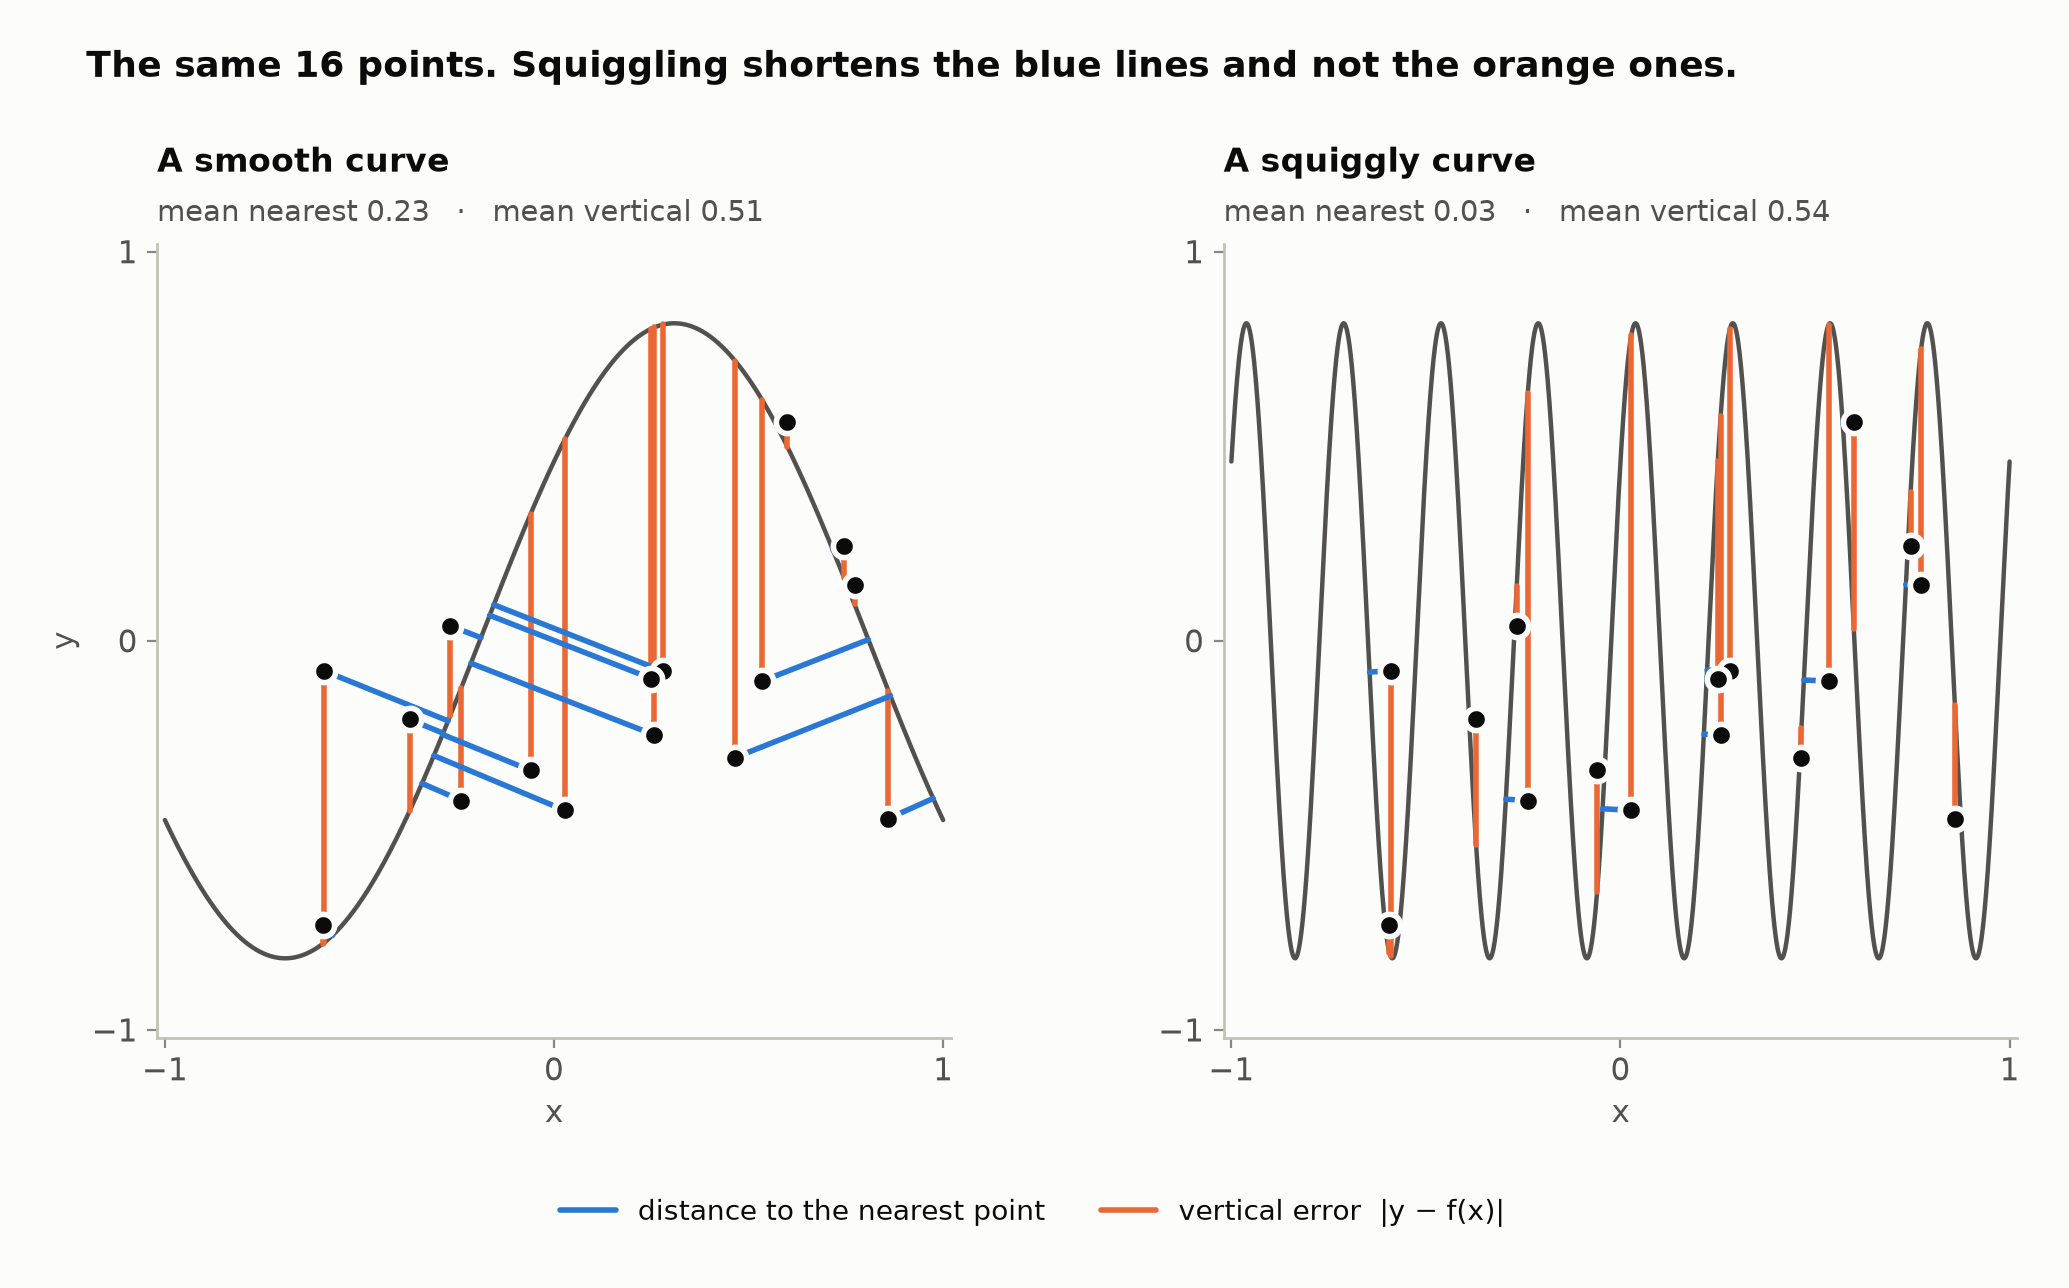
\includegraphics[width=0.78\linewidth]{../graphs/readme_two_distances.png}
  \caption{The two distances, on the same 16 points. Blue: distance to the
  nearest point of the curve. Orange: vertical error $|y-f(x)|$. Raising the
  frequency of the sine from 1 (left) to 8 (right) shortens the blue segments
  and leaves the orange ones as long as before.}
  \label{fig:two}
\end{figure}

\paragraph{Results.} (G) is true, (P) is false for width and holds weakly for
depth, and (L) is false.
\begin{itemize}\setlength{\itemsep}{0pt}
\item \emph{Slope sandwich} (\cref{thm:sandwich}). For a $K$-Lipschitz function
and any data point, $\text{vertical}/\sqrt{1+K^2}\le\text{nearest}\le\text{vertical}$.
The curve can be much nearer than its vertical error only where it is steep.
\item \emph{Marginal lemma} (\cref{thm:marginal}). The expected loss of a random
function, for any loss of the residual $y-f(x)$, depends only on the
distribution of $f(x)$ at each single $x$. For random-phase waves this
distribution does not depend on the frequency (\cref{cor:phase}), and for ReLU
networks under He initialisation the expected initial squared error does not
depend on the width (\cref{cor:he}).
\item \emph{Tube identity and length bound} (\cref{thm:tube,prop:length}). The
mean distance from a random point to a set is the mass outside the tube of
radius $r$ around the set, integrated over $r$. For a curve of length $l$ and a
uniform point in a planar region of area $V$ it is at least
$V/(4l+2\sqrt{\pi V})$.
\item \emph{The sine} (\cref{prop:sine,prop:floor}). For a sine that spans the
data, distance times frequency tends to $(2-8/\pi^2)/4\approx0.2974$. With a
smaller amplitude the distance stops at a floor set by the amplitude, not by
the number of points.
\item \emph{Experiments} (\cref{sec:experiments}). With amplitude and marginals
held fixed, the nearest-point distance falls from $0.613$ to $0.021$ while the
vertical error stays between $0.665$ and $0.669$. Random ReLU networks have the
predicted, width-independent initial squared error, and their curves are not
longer at larger width.
\end{itemize}

\paragraph{Scope.} This is a negative result about one intuitive picture. An
earlier draft of this paper claimed empirical support for the conjecture; that
support came from faulty measurement code, and the draft was withdrawn
(\cref{app:wrong}). The individual statements here are elementary, and we make
no claim of priority for any of them; \cref{sec:related} lists the work we are
aware of. \Cref{thm:sandwich,thm:marginal,thm:tube} and \cref{cor:phase} are
formalised in Lean~4 (\cref{sec:lean}). Code, the Lean project and the
development notes are at \repo.

\section{Setting and results}
\label{sec:theory}

\subsection{Two distances}

Let $(X,d)$ be a metric space of inputs and $f:X\to\R$ a function. A data point
is a pair $(x,y)\in X\times\R$. We give $X\times\R$ the Euclidean product metric
$\rho\bigl((x,y),(x',y')\bigr)=\sqrt{d(x,x')^2+(y-y')^2}$ and write
$\Gamma_f=\{(x,f(x)):x\in X\}$ for the graph of $f$, the ``line'' of the
conjecture. Two quantities compare a data point with the line:
\begin{align*}
  \vd_f(x,y) &= |y-f(x)| && \text{(vertical error)},\\
  \nd_f(x,y) &= \inf_{x'\in X}\rho\bigl((x,y),(x',f(x'))\bigr) && \text{(nearest-point distance)}.
\end{align*}
Regression losses are functions of the residual $y-f(x)$, so they see $\vd_f$.
The conjecture is stated with $\nd_f$.

A \emph{random function} $F$ is a probability space $(\Theta,\pi)$ of parameters
together with functions $f_\theta:X\to\R$ such that $\theta\mapsto f_\theta(x)$
is measurable for every $x$. Its \emph{one-point marginal} at $x$ is the law
$\nu^F_x$ of $f_\theta(x)$ under $\pi$. For a cost $c$ and a data distribution
$\mu$ on $X\times\R$, the expected cost at initialisation is
$\E_{(x,y)\sim\mu}\,\E_{\theta\sim\pi}\,c(f_\theta;x,y)$.\footnote{We assume the
inner expectation is a measurable function of $(x,y)$. This holds if
$(\theta,x)\mapsto f_\theta(x)$ is jointly measurable, and always when $\mu$ is
the empirical measure of a finite data set.} For a family of random functions
indexed by a size $m$, ``a bigger model starts closer'' means that this
expectation is strictly decreasing in $m$. Claim (G) uses the cost $\nd$ and
claim (L) uses costs of the form $\ell(y-f(x))$. We make ``squiggly'' concrete
by the frequency of a wave of fixed amplitude and, for networks, by arc length
and the number of turns.

\subsection{The slope sandwich}

\begin{theorem}[Slope sandwich]\label{thm:sandwich}
If $f$ is $K$-Lipschitz, then for every data point $(x,y)$
\[
  \frac{\vd_f(x,y)}{\sqrt{1+K^2}}\;\le\;\nd_f(x,y)\;\le\;\vd_f(x,y).
\]
\end{theorem}

\begin{proof}
The point $(x,f(x))$ lies on $\Gamma_f$ at distance $|y-f(x)|$ from $(x,y)$,
which gives the upper bound. For the lower bound take any $x'\in X$ and put
$a=d(x,x')$ and $b=|y-f(x')|$. By the triangle inequality and the Lipschitz
bound, $|y-f(x)|\le|y-f(x')|+|f(x')-f(x)|\le b+Ka$. By the Cauchy--Schwarz
inequality, $b+Ka\le\sqrt{1+K^2}\,\sqrt{a^2+b^2}=\sqrt{1+K^2}\;\rho\bigl((x,y),(x',f(x'))\bigr)$.
Taking the infimum over $x'$ gives $\vd_f(x,y)\le\sqrt{1+K^2}\,\nd_f(x,y)$.
\end{proof}

Both bounds are attained: for $X=\R$ and $f(x)=Kx$, the point $(0,y)$ has
$\nd_f=|y|/\sqrt{1+K^2}$, and for a constant $f$ the two distances coincide.
Taking expectations, the same two inequalities hold between the mean distances
of any random $K$-Lipschitz function and any data distribution.

The theorem says what a small nearest-point distance means. If
$\nd_f(x,y)<\eta$, there is an input $x'$ with $d(x,x')<\eta$ and
$|y-f(x')|<\eta$: a perturbation of the \emph{input} smaller than $\eta$ brings
the output within $\eta$ of the label. When $\nd_f$ is small and $\vd_f$ is not,
the function is steep near $x$: its Lipschitz constant is at least
$\sqrt{(\vd_f/\nd_f)^2-1}$. That describes a function that is
sensitive to its input near the data, not one that fits the data.

\subsection{The marginal lemma}

\begin{theorem}[Marginal lemma]\label{thm:marginal}
Let $F$ be a random function and $\ell:\R\to[0,\infty)$ a measurable loss. For
every data point $(x,y)$,
\[
  \E_{\theta}\,\ell\bigl(y-f_\theta(x)\bigr)=\int_{\R}\ell(y-t)\,\nu^F_x(dt).
\]
Consequently, if two random functions $F$ and $G$ have $\nu^F_x=\nu^G_x$ for
every $x$, their expected losses are equal for every such $\ell$ and every data
distribution $\mu$.
\end{theorem}

\begin{proof}
By definition $\nu^F_x$ is the image of $\pi$ under $\theta\mapsto f_\theta(x)$.
The displayed identity is the change-of-variables formula for an image measure,
applied to the measurable function $t\mapsto\ell(y-t)$. Integrating both sides
against $\mu$ gives the second statement.
\end{proof}

The proof is one line, and the content is in what is absent: the joint law of
$\bigl(f_\theta(x),f_\theta(x')\bigr)$ at two inputs does not enter. How $f$
moves between inputs is what ``squiggly'' means, so the expected initial loss
cannot register squiggliness. The lemma is about the expectation over $\theta$
only. The variance of the initial loss, the probability of a low initial loss,
and everything that happens during training do depend on joint laws.

\begin{corollary}[Random-phase waves]\label[corollary]{cor:phase}
Let $g:\R\to\R$ be measurable and $T$-periodic, let $\varphi$ be uniform on
$[0,T)$, and for a frequency $w\in\R$ let $f_{w,\varphi}(x)=g(wx+\varphi)$ on
$X=\R$. Then the one-point marginal of $f_{w,\cdot}$ at every $x$ is the law of
$g(\varphi)$, for every $w$. Hence the expected loss
$\E_{(x,y)\sim\mu}\E_\varphi\,\ell\bigl(y-f_{w,\varphi}(x)\bigr)$ is the same for
every $w$, every measurable $\ell\ge0$ and every $\mu$. No sequence of
frequencies makes it decrease.
\end{corollary}

\begin{proof}
The uniform distribution on the circle $\R/T\mathbb{Z}$ is invariant under
translation, so $wx+\varphi \bmod T$ is uniform on $[0,T)$ for every fixed $w$
and $x$, and $g(wx+\varphi)$ has the law of $g(\varphi)$. Apply
\cref{thm:marginal}.
\end{proof}

For the curves of \cref{sec:experiments}, $g=p\sin$ with peak $p\le1$, and data
with $y$ uniform on $[-1,1]$ independent of $x$. Since
$\E_y|y-s|=(1+s^2)/2$ for $|s|\le1$, the expected vertical error is
$(1+p^2/2)/2$ at every frequency.

\begin{corollary}[ReLU networks under He initialisation]\label[corollary]{cor:he}
Let $f_\theta(x)=u^\top\relu\bigl(W^L\relu(\cdots\relu(W^1x))\bigr)$ for
$x\in\R^{d}$, with $\relu$ the ReLU, no biases, hidden widths $n_1,\dots,n_L$,
$n_0=d$, and independent weights $W^k_{ij}\sim N(0,2/n_{k-1})$ and
$u_i\sim N(0,2/n_L)$. Then for every $x$ and $y$,
\[
  \E f_\theta(x)=0,\qquad \E f_\theta(x)^2=\frac{2\|x\|^2}{d},\qquad
  \E\bigl(y-f_\theta(x)\bigr)^2=y^2+\frac{2\|x\|^2}{d},
\]
whatever the depth and the widths. If all weights are instead $N(0,1)$, the last
quantity is $y^2+\|x\|^2\prod_{k=1}^{L}(n_k/2)$.
\end{corollary}

The proof is a layer-by-layer recursion for $\E\|h^k\|^2$ and is in
\cref{app:proofs}. It uses only that the weights are independent, symmetric and
of the stated variance; preserving the second moment across layers is the
design criterion of this initialisation \citep{he2015delving}. In the terms of
\cref{thm:marginal}, the squared loss reads only the first two moments of
$\nu_x$, and these do not depend on the width. The full law $\nu_x$ does depend
on the width, so for other losses the corollary gives no exact statement.

\subsection{The tube identity and a bound from length}

For a non-empty set $S$ in a metric space, write
$N_r(S)=\{q:\dist(q,S)\le r\}$ for the closed tube of radius $r$ around $S$.

\begin{theorem}[Tube identity]\label{thm:tube}
Let $S$ be a non-empty subset of a metric space and $P$ a random point of that
space. Then
\[
  \E\,\dist(P,S)=\int_0^\infty\P\bigl(\dist(P,S)>r\bigr)\,dr
  =\int_0^\infty\P\bigl(P\notin N_r(S)\bigr)\,dr ,
\]
where both sides may be infinite.
\end{theorem}

\begin{proof}
The function $q\mapsto\dist(q,S)$ is $1$-Lipschitz, hence measurable, and
non-negative. For a non-negative random variable $Z$ we have
$Z=\int_0^\infty\mathbf 1\{Z>r\}\,dr$, and Tonelli's theorem gives
$\E Z=\int_0^\infty\P(Z>r)\,dr$. This is the layer-cake formula
\citep[Section~1.13]{lieb2001analysis}. Take $Z=\dist(P,S)$.
\end{proof}

The identity holds for any set in any metric space. It reduces the mean
distance to the volume of tubes, which for curves in the plane is controlled by
length.

\begin{lemma}\label[lemma]{lem:tube-area}
Let $S\subset\R^2$ be the image of a rectifiable curve of length $l$. Then the
area of $N_r(S)$ is at most $2lr+\pi r^2$ for every $r\ge0$.
\end{lemma}

The proof, by polygonal approximation, is in \cref{app:proofs}.

\begin{proposition}[Length bound]\label[proposition]{prop:length}
Let $\Omega\subset\R^2$ be measurable with area $V\in(0,\infty)$, let $P$ be
uniform on $\Omega$, and let $S$ be the image of a rectifiable curve of length
$l$. Then
\[
  \E\,\dist(P,S)\;\ge\;\frac{V}{4l+2\sqrt{\pi V}} .
\]
\end{proposition}

\begin{proof}
Put $r_0=V/(2l+\sqrt{\pi V})$. For $0\le r\le r_0$ we have
$\pi r\le\pi V/\sqrt{\pi V}=\sqrt{\pi V}$, so by \cref{lem:tube-area} the area
of $N_r(S)$ is at most $(2l+\sqrt{\pi V})\,r=Vr/r_0$. Therefore
$\P(P\notin N_r(S))\ge1-r/r_0$ for $r\le r_0$, and by \cref{thm:tube}
$\E\,\dist(P,S)\ge\int_0^{r_0}(1-r/r_0)\,dr=r_0/2$.
\end{proof}

To leading order in $l$ the bound is $V/(4l)$. We draw three consequences.
Length is necessary: a mean distance of at most $\varepsilon$ requires
$l\ge V/(4\varepsilon)-\sqrt{\pi V}/2$. Length is not sufficient: a part of the
curve further than $r$ from $\Omega$ adds nothing to $N_r(S)\cap\Omega$, so
length outside the data region is wasted (\cref{sec:line}). And the bound is
nearly attained only if the tube around the curve stays inside $\Omega$ and
overlaps itself little, that is, if the length is spread evenly over the
region. The proposition is for curves in the plane; for inputs of dimension
above one the graph is a surface, and its area takes the role of length.

\subsection{The sine family}

The experiments use $f_{w,\varphi}(x)=p\sin(w\pi x+\varphi)$ on $x\in[-1,1]$
with $\varphi$ uniform on $[0,2\pi)$, and a point $P$ uniform on
$\Omega=[-1,1]^2$, so $V=4$. The curve makes $w$ full periods across the box and
is $p\,w\pi$-Lipschitz. Write $D_p(w)$ for the mean of $\nd$ over $P$ and
$\varphi$, and $l(w)$ for the arc length.

\begin{proposition}[The sine that spans the data; leading order]\label[proposition]{prop:sine}
For $p=1$, as $w\to\infty$,
\[
  \frac{l(w)}{w}\to4,\qquad
  w\,D_1(w)\to\frac{2-8/\pi^2}{4}\approx0.2974,\qquad
  D_1(w)\,l(w)\to2-\frac{8}{\pi^2}\approx1.189 .
\]
\end{proposition}

The first limit is proved in \cref{app:proofs}. The second is a leading-order
derivation. At height $y$ the curve crosses on two interleaved lattices of
period $2/w$, with gaps $(1/w)(1\mp2\arcsin(y)/\pi)$. At high frequency the
strokes are nearly vertical, so the nearest point of the curve is, to leading
order, the nearest crossing at the same height. Averaging that distance over
$x$ and then over $y$, with $\int_0^1\arcsin(y)^2\,dy=\pi^2/4-2$, gives the
constant. The step from horizontal to Euclidean distance is argued in outline
in \cref{app:proofs}, without all details, and the constant is checked
numerically in \cref{sec:saturation}. The limit $1.189$ exceeds the value
$V/4=1$ of \cref{prop:length} because the strokes of a sine are not evenly
spaced.

\begin{proposition}[Band-edge floor]\label[proposition]{prop:floor}
For $0<p\le1$ and $w\ge1$,
\[
  \frac{(1-p)^2}{2}\;\le\;D_p(w)\;\le\;\frac{(1-p)^2}{2}+\frac{2}{w}.
\]
\end{proposition}

The proof is in \cref{app:proofs}. The curve stays in the band $|y|\le p$, so a
point at height $|y|>p$ is never nearer than $|y|-p$, and
$\E\max(0,|y|-p)=(1-p)^2/2$. Raising the frequency removes the rest at rate
$O(1/w)$. The floor depends on the amplitude relative to the range of the data.
It does not depend on the number of data points: $D_p(w)$ is the mean of a
per-point quantity, so its expectation is the same for a sample of any size.

\subsection{The covering bound and the theorem for sines}
\label{sec:cover}

The upper bound in \cref{prop:floor} is an instance of a general fact, which
says what a function must do to be near the data.

\begin{definition}[Covering]\label[definition]{def:cover}
A function $f:X\to\R$ \emph{covers} a set of labels $S\subset\R$ \emph{within}
$\rho$ if for every $x\in X$ and every $y\in S$ there is an $x'\in X$ with
$d(x,x')\le\rho$ and $f(x')=y$.
\end{definition}

The smallest such $\rho$ is an oscillation scale: how far one must move in the
input to see every label.

\begin{theorem}[Covering bound]\label{thm:cover}
If $f$ covers $S$ within $\rho$, then $\nd_f(x,y)\le\rho$ for every data point
with $y\in S$. If in addition $f$ is $K$-Lipschitz, then
$\vd_f(x,y)\le\sqrt{1+K^2}\,\rho$ for every such point.
\end{theorem}

\begin{proof}
Take $x'$ as in \cref{def:cover}. The point $(x',y)=(x',f(x'))$ lies on
$\Gamma_f$ at distance $d(x,x')\le\rho$ from $(x,y)$. The second statement
follows from \cref{thm:sandwich}.
\end{proof}

\begin{corollary}[Nearness is a distance to move]\label[corollary]{cor:warp}
If $f$ covers $S$ within $\rho$, then for every target $g:X\to S$ there is a map
$h:X\to X$ with $d(x,h(x))\le\rho$ for every $x$ and $f\circ h=g$.
\end{corollary}

\begin{proof}
For each $x$ choose $h(x)$ as the point $x'$ of \cref{def:cover} for the label
$g(x)$.
\end{proof}

The corollary says in what sense the nearness can be used. The loss at
initialisation does not see it (\cref{thm:marginal}). But a function that
covers the labels within $\rho$ fits any data with labels in $S$ once each
input is moved by at most $\rho$. For a single data point the movement is a
shift, which for a wave is a change of phase. For several points the shifts
differ, and $h$ is a warp of the input, which in a network is what the earlier
layers can supply. The corollary does not say that $h$ is continuous, or that
training finds it.

So a small oscillation scale is sufficient for a small nearest-point distance,
and by the second statement of \cref{thm:cover} it has a price: a function that covers labels at
vertical distance $\vd$ within $\rho$ has slope at least
$\sqrt{(\vd/\rho)^2-1}$. Claims (G) and (P) for a family of models therefore
come down to how its oscillation scale and its slope depend on its size. For
sines both are explicit.

The sine is one case of a statement about any function. For a function $f$ on
a normed space $X$ and $w>0$, write $f_w(x)=f(wx)$ for $f$ squeezed sideways by
the factor $w$.

\begin{theorem}[The squiggly line theorem]\label{thm:general}
Let $F$ be a random function on a normed space $X$ such that every draw
$f_\theta$ covers $S$ within $\rho$ and is $K$-Lipschitz, and such that the
one-point marginal $\nu^F_x$ is the same at every $x$. Let $F_w$ be $F$ with
every draw squeezed by $w>0$.
\begin{enumerate}\setlength{\itemsep}{0pt}
\item[(i)] \emph{Closer and steeper.} For every draw and every data point with
$y\in S$,
$\vd/\sqrt{1+(wK)^2}\le\nd\le\rho/w$.
\item[(ii)] For a probability measure $\mu$ on data points with $y\in S$ almost
surely, the expected nearest-point distance of $F_w$ is at most $\rho/w$ and
tends to $0$ as $w\to\infty$.
\item[(iii)] \emph{No better at the start.} For every measurable loss
$\ell\ge0$, the expected loss of $F_w$ is the same for every $w$.
\item[(iv)] For every target $g:X\to S$ and every draw there is a map $h$ with
$d(x,h(x))\le\rho/w$ and $f_{\theta,w}\circ h=g$.
\end{enumerate}
\end{theorem}

\begin{proof}
If $f$ covers $S$ within $\rho$ then $f_w$ covers $S$ within $\rho/w$: given
$x$ and $y$, take $z$ with $\|wx-z\|\le\rho$ and $f(z)=y$, and put $x'=z/w$.
If $f$ is $K$-Lipschitz then $f_w$ is $wK$-Lipschitz. So (i) is
\cref{thm:sandwich,thm:cover}, (ii) follows from (i), and (iv) is
\cref{cor:warp}. For (iii), the marginal of $F_w$ at $x$ is $\nu^F_{wx}$, which
does not depend on $w$ or $x$; apply \cref{thm:marginal}.
\end{proof}

No part of the statement uses the dimension of $X$ or a period. For the sine
the constants are explicit.

\begin{theorem}[The squiggly line theorem, for sines]\label{thm:sine}
Let $X=\R$, $p>0$ and $w>0$, and let $f_{w,\varphi}(x)=p\sin(w\pi x+\varphi)$.
\begin{enumerate}\setlength{\itemsep}{0pt}
\item[(i)] For every phase $\varphi$ and every data point $(x,y)$ with
$|y|\le p$,
\[
  \frac{\vd_{f_{w,\varphi}}(x,y)}{\sqrt{1+(p\,w\pi)^2}}\;\le\;\nd_{f_{w,\varphi}}(x,y)\;\le\;\frac1w .
\]
\item[(ii)] If $\mu$ is a probability measure on data points with $|y|\le p$
almost surely and $\varphi$ is uniform on $[0,2\pi)$, the expected
nearest-point distance is at most $1/w$, and tends to $0$ as $w\to\infty$.
\item[(iii)] For every measurable loss $\ell\ge0$ and every $\mu$, the expected
loss $\E_{(x,y)\sim\mu}\E_\varphi\,\ell\bigl(y-f_{w,\varphi}(x)\bigr)$ is the
same for every $w$.
\end{enumerate}
\end{theorem}

\begin{proof}
(i) The function is $p\,w\pi$-Lipschitz, which gives the lower bound by
\cref{thm:sandwich}. For the upper bound we show that it covers $[-p,p]$ within
$1/w$. Given $x$ and $y$ with $|y|\le p$, put $t=\arcsin(y/p)$ and
$\theta_0=w\pi x+\varphi$, let $k$ be an integer nearest to
$(\theta_0-t)/(2\pi)$, and put $\theta=t+2\pi k$. Then $|\theta-\theta_0|\le\pi$.
The input $x'=(\theta-\varphi)/(w\pi)$ satisfies $|x-x'|=|\theta-\theta_0|/(w\pi)\le1/w$
and $f_{w,\varphi}(x')=p\sin t=y$. Apply \cref{thm:cover}.
(ii) The bound in (i) holds for every phase and almost every data point, and
$\nd\ge0$. (iii) is \cref{cor:phase}.
\end{proof}

Parts (i) and (ii) are claim (G), with a rate: both ends of the sandwich fall
like $1/w$. Part (iii) is the failure of claim (L). By \cref{cor:warp}, any
target with values in $[-p,p]$ is fitted exactly by $f_{w,\varphi}$ after a warp
of the input of size at most $1/w$. For one data point this is a change of
phase of at most $\pi$, at every frequency: a squigglier sine is closer in the
input and exactly as far in the phase. On the bounded domain
$[-1,1]$ of the experiments the same argument gives $2/w$ in place of $1/w$,
which is the upper bound of \cref{prop:floor}; the exact constant is the one in
\cref{prop:sine}.

\section{Experiments}
\label{sec:experiments}

All experiments are small numerical computations with our own scripts
(\cref{app:details} lists them). Unless stated otherwise, curves are
$f(x)=A\sqrt2\,\sin(w\pi x+\varphi)$ on $[-1,1]$ and data points are uniform on
$[-1,1]^2$, with $y$ independent of $x$. The default amplitude is $A=0.577$, the
standard deviation of the labels, so the peak is $p=A\sqrt2=0.816$. Each curve
is sampled as a polyline with consecutive samples at most $0.002$ apart along
the curve, and the distance from a point to the polyline is computed exactly.

\subsection{Frequency with everything else held fixed}
\label{sec:freq}

Earlier tests of the conjecture varied polynomial degree or network width, which
changes the output amplitude together with the squiggliness. Here the frequency
$w$ is the only variable: by \cref{cor:phase} the distribution of $f(x)$ at
every $x$ is identical in every row of \cref{tab:freq}. We use 3000 trials of
30 points each and 100 stratified random phases per frequency.

\begin{table}[t]
  \caption{Frequency isolation. Mean nearest-point distance and mean vertical
  error against frequency $w$, with the two lower bounds on the nearest-point
  distance: the mean vertical error divided by $\sqrt{1+K^2}$ with $K=p\,w\pi$
  (\cref{thm:sandwich}), and $4/(4l+4\sqrt\pi)$ (\cref{prop:length} with $V=4$).}
  \label{tab:freq}
  \centering
  \begin{tabular}{rrcccc}
    \toprule
    $w$ & arc length $l$ & nearest-point & vertical & bound, \cref{thm:sandwich} & bound, \cref{prop:length} \\
    \midrule
    0.25 &   2.19 & 0.6129 & 0.6672 & 0.5617 & 0.2524 \\
    0.5  &   2.66 & 0.4890 & 0.6664 & 0.4099 & 0.2256 \\
    1    &   3.96 & 0.3095 & 0.6649 & 0.2416 & 0.1744 \\
    2    &   6.96 & 0.1717 & 0.6651 & 0.1273 & 0.1145 \\
    4    &  13.32 & 0.0928 & 0.6663 & 0.0647 & 0.0663 \\
    8    &  26.26 & 0.0529 & 0.6678 & 0.0325 & 0.0357 \\
    16   &  52.31 & 0.0338 & 0.6665 & 0.0162 & 0.0185 \\
    32   & 104.50 & 0.0249 & 0.6657 & 0.0081 & 0.0094 \\
    64   & 208.92 & 0.0207 & 0.6688 & 0.0041 & 0.0047 \\
    \bottomrule
  \end{tabular}
\end{table}

\begin{figure}[t]
  \centering
  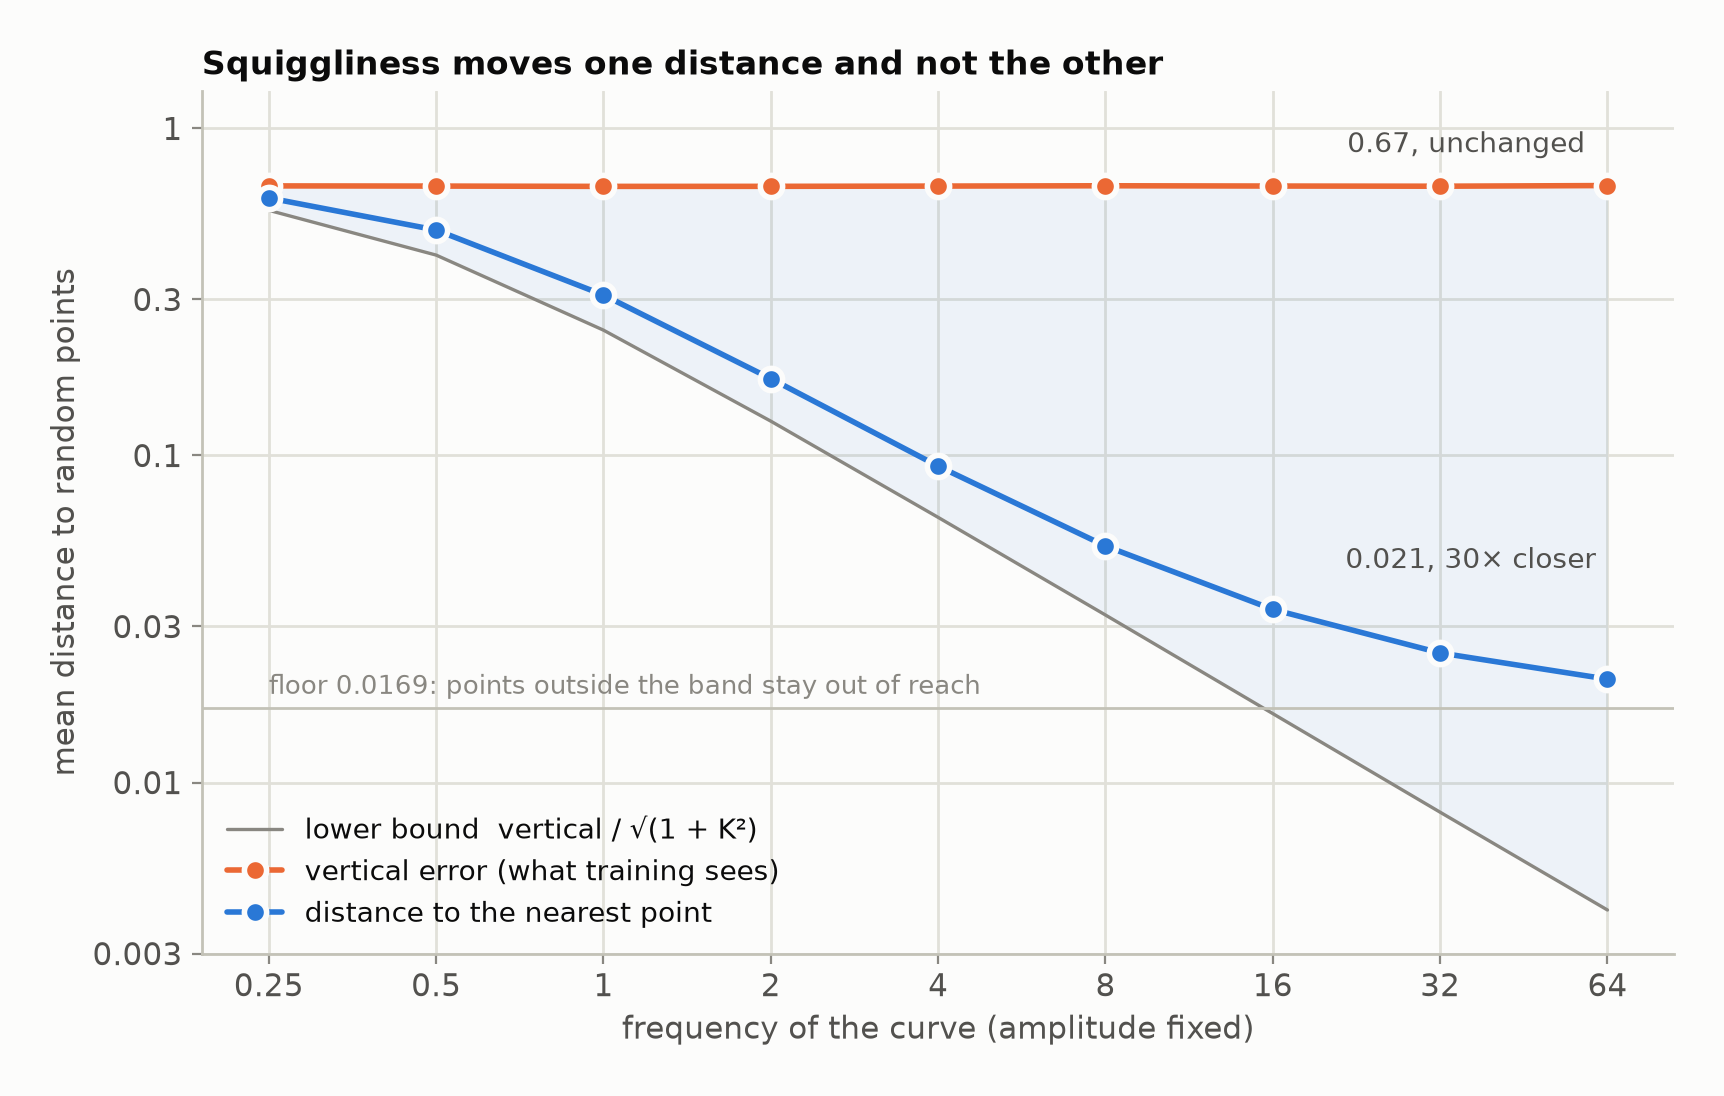
\includegraphics[width=0.72\linewidth]{../graphs/readme_frequency.png}
  \caption{The data of \cref{tab:freq}. The nearest-point distance (blue) falls
  with frequency and stays above the lower bound of \cref{thm:sandwich} (grey
  line). The vertical error (orange) does not move. The horizontal line is the
  floor $(1-p)^2/2=0.0169$ of \cref{prop:floor}.}
  \label{fig:freq}
\end{figure}

The nearest-point distance falls from $0.6129$ to $0.0207$, a factor of $29.6$.
Claim (G) holds, and not through amplitude. The vertical error lies between
$0.6649$ and $0.6688$ in every row, with no trend; the value predicted after
\cref{cor:phase} is $(1+p^2/2)/2=0.6665$. The flat column is \cref{cor:phase}
observed, and the differences between rows are sampling noise. Both lower bounds
hold in every row. At $w=64$ the function has Lipschitz constant $164$, and this
steepness is what \cref{thm:sandwich} requires for a nearest-point distance 32
times smaller than the vertical error. From $w=16$ the gap to both bounds
widens, because the distance approaches the floor of \cref{prop:floor}
(\cref{fig:freq}).

\subsection{A straight line of the same length}
\label{sec:line}

If length alone produced the effect, a straight segment of the same arc length
should score like the sine. We take $y=mx+b$ on $x\in[-1,1]$ with
$m=\sqrt{(l/2)^2-1}$, so that its length is $l$, and $b$ uniform on $[-1,1]$.

\begin{table}[t]
  \caption{Mean nearest-point distance for the sine and for a straight segment
  of the same length. The last two columns give the slope of the segment and
  the share of its length that lies outside the data box $[-1,1]^2$, averaged
  over $b$.}
  \label{tab:line}
  \centering
  \begin{tabular}{rrccrc}
    \toprule
    $w$ & arc length & sine & straight segment & slope $m$ & share outside the box \\
    \midrule
    4  &  13.32 & 0.0928 & 0.5022 &   6.6 & 85\% \\
    16 &  52.31 & 0.0338 & 0.5007 &  26.1 & 96\% \\
    64 & 208.92 & 0.0207 & 0.5006 & 104.5 & 99\% \\
    \bottomrule
  \end{tabular}
\end{table}

The segment stays at $0.50$ while the sine reaches $0.021$ (\cref{tab:line}).
This comparison needs a caveat. A segment of length $209$ over $x\in[-1,1]$ has
slope $104$, and about $99\%$ of it lies above or below the data. The part
inside the box has length about $2$ in all three rows, and a near-vertical
segment of length $2$ through the middle of the box has mean distance
$\E|x|=0.5$. The table therefore shows that length outside the data region is
worth nothing. It does not show that length is irrelevant: by
\cref{prop:length}, length is necessary, and the sine achieves its small
distance because its length is inside the box and spread across it.

\subsection{What sets the floor}
\label{sec:saturation}

An earlier version of this work predicted that the distance stops falling once
the wavelength $2/w$ drops below the mean spacing $2/n$ of $n$ data points, so
that the knee of the curve $D(w)$ would sit at $w^\ast\propto n$. We swept
$n\in\{10,30,100,300,1000\}$ and 25 frequencies in $[1,1000]$ with $30\,000$
points per $n$, and located the knee by two criteria fixed in advance: the
breakpoint of a continuous two-segment fit of $\log D$ on $\log w$, and the
smallest $w$ at which doubling $w$ lowers $D$ by less than $10\%$.

\begin{table}[t]
  \caption{Knee frequency $w^\ast$ against the number of points $n$. The
  prediction under test was slope $1$ of $\log w^\ast$ on $\log n$. Confidence
  intervals are from a bootstrap over trials.}
  \label{tab:knee}
  \centering
  \begin{tabular}{lcccccrc}
    \toprule
    criterion & $n=10$ & 30 & 100 & 300 & 1000 & slope & 95\% interval \\
    \midrule
    two-segment fit      & 21.6 & 21.6 & 21.6 & 21.6 & 21.6 & $-0.000$ & $[-0.004,\,0.004]$ \\
    doubling gains $<10\%$ & 60.1 & 61.7 & 61.4 & 61.0 & 59.4 & $-0.003$ & $[-0.014,\,0.008]$ \\
    \bottomrule
  \end{tabular}
\end{table}

The slope is $0$, not $1$ (\cref{tab:knee}), and the five curves $D(w)$ agree to
within $3.1\%$ at every frequency. No experiment was needed for this: the
quantity is a mean of per-point distances, so its expectation cannot depend on
$n$. What sets the knee is the band edge of \cref{prop:floor}. With $p=0.816$
the floor is $D_\infty=(1-p)^2/2=0.0169$, and a fit of
$D-D_\infty=c\,w^{-\beta}$ for $w\ge20$ gives $\beta=0.990$ and $c=0.248$. For
$D=D_\infty+c/w$ the $10\%$ criterion triggers at $c(1-2r)/(2rD_\infty)=58.6$
with $r=0.1$, against $59$ to $62$ measured.

As a control we set $A\sqrt2=1$, so that the band covers the data and the floor
is zero. The saturation disappears (\cref{fig:floor}): the distance follows
$0.301\,w^{-1.002}$ up to $w=1000$, where it is $0.00030$, and the $10\%$
criterion never triggers.\footnote{The two-segment fit still reports a
breakpoint, at $1.8$, because it always returns one.} \Cref{prop:sine} predicts
$w\,D_1(w)\to0.2974$. The repository reports $0.2965$ at $w=256$; a separate run
for this paper, with $40\,000$ points and 8 phases, gave $0.298$ at $w=64$ and
at $w=256$, and $D\,l=1.192$ against the predicted $1.189$.

\begin{figure}[t]
  \centering
  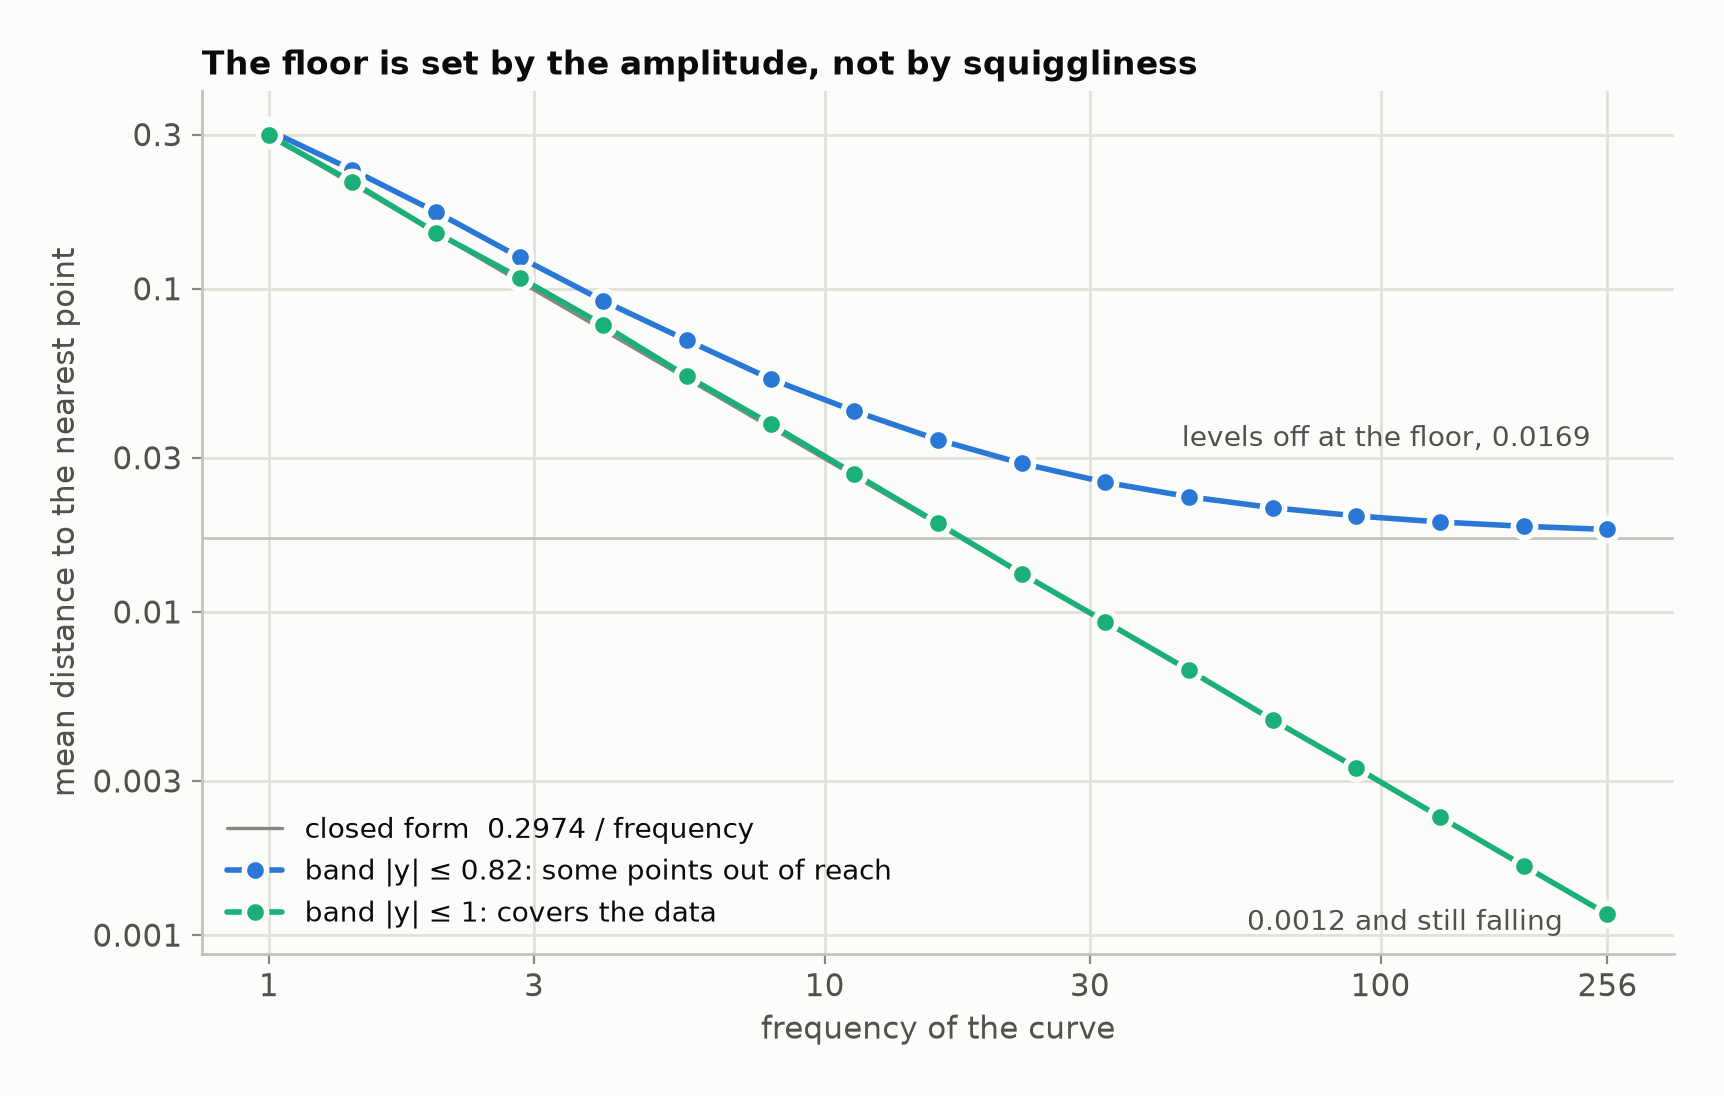
\includegraphics[width=0.72\linewidth]{../graphs/readme_floor.png}
  \caption{The floor comes from the amplitude. Blue: default amplitude, band
  $|y|\le0.82$; the distance levels off at $0.0169$. Green: band $|y|\le1$; no
  floor, and the distance follows the constant of \cref{prop:sine} (grey line,
  under the green one).}
  \label{fig:floor}
\end{figure}

\subsection{Random networks}
\label{sec:nets}

\paragraph{Initial loss against width.} We draw 200 points with $x$ uniform on
$[-1,1]^{10}$ and $y$ uniform on $[-1,1]$, and for each width 200 untrained
ReLU networks with two hidden layers and no biases, as in \cref{cor:he}. The
prediction of \cref{cor:he}, evaluated on the sample, is the mean of
$y^2+2\|x\|^2/d$, which is $1.03$.

\begin{table}[t]
  \caption{Mean squared error before training, 200 networks per width
  ($\pm$ one standard error). Predictions are from \cref{cor:he}.}
  \label{tab:mse}
  \centering
  \begin{tabular}{rcccc}
    \toprule
    & \multicolumn{2}{c}{He initialisation} & \multicolumn{2}{c}{$N(0,1)$ weights} \\
    \cmidrule(lr){2-3}\cmidrule(lr){4-5}
    width & measured & predicted & measured & predicted \\
    \midrule
       4 & $1.07\pm0.12$ & 1.03 & $15$ & $14$ \\
      16 & $1.02\pm0.05$ & 1.03 & $220$ & $219$ \\
      64 & $1.07\pm0.04$ & 1.03 & $3.45\times10^{3}$ & $3.51\times10^{3}$ \\
     256 & $1.10\pm0.04$ & 1.03 & $6.02\times10^{4}$ & $5.61\times10^{4}$ \\
    1024 & $1.03\pm0.04$ & 1.03 & $8.23\times10^{5}$ & $8.97\times10^{5}$ \\
    \bottomrule
  \end{tabular}
\end{table}

A wider network does not start closer (\cref{tab:mse}; \cref{fig:mse} in \cref{app:details}). The measured
values scatter around the prediction; the largest deviation, at width 256, is
$1.9$ standard errors. With unscaled weights a wider network starts much further
away, because its output grows with width. That growth is an amplitude effect,
and it is the confound that the design of \cref{sec:freq} removes.

\paragraph{Curve length against width and depth.} For claim (P) we look at the
curves themselves, for a one-dimensional input. Each network has He-uniform
weights and hidden biases uniform on $[-0.5,0.5]$, and its output is shifted and
scaled so that its range over $[-1,1]$ is exactly $[-1,1]$. We measure arc
length, the number of turns (sign changes of the slope), and the mean
nearest-point distance to 200 fixed random points, over 300 networks per size.

Width adds turns and no length (\cref{tab:relu-full} in \cref{app:details}).
From width 2 to 512, with two hidden layers, the mean number of turns rises
from $0.5$ to $15$, the arc length stays between $3.4$ and $3.6$, and the
nearest-point distance is flat from width 16, between $0.42$ and $0.43$. Depth
adds some length: from 1 to 16 layers at width 64 the arc length rises from
$3.4$ to $5.1$ and the distance falls from $0.44$ to $0.34$. For comparison,
the same code gives length $4.61$ and distance $0.351$ for a sine with one
period across the box, and $64.07$ and $0.021$ for a sine with 16 periods. Even
at depth 16 the random curves resemble the first and not the second. So claim
(P) fails for width and holds weakly for depth.

This measurement has caveats. The input is one-dimensional. Rescaling the output
controls the amplitude but does not hold the marginals of $f(x)$ fixed, unlike
\cref{sec:freq}. Only the nearest-point distance is measured, not the vertical
error. The distances use a fixed grid of 4001 samples, which overestimates the
distance by about $7\%$ for the sine with 16 periods ($0.0209$ against $0.0196$
with exact projection). Finally, the rescaling and the biases mean that the
depth trend is not directly comparable with the theorem of
\citet{hanin2022preserve} discussed in \cref{sec:related}.

\section{Formalisation}
\label{sec:lean}

The repository contains a Lean~4 project \citep{demoura2021lean4} on Mathlib
\citep{mathlib2020} that states the conjecture and proves the results that
refute claim (L). A randomly initialised model is a parameter type with a
probability measure and an evaluation map, and one definition says that the
expected cost is strictly decreasing in the size of the model; the conjecture
and the learning claim are that definition for the nearest-point distance and
for a loss of the residual. Proved: \cref{thm:sandwich}, for inputs in any
seminormed group; \cref{thm:tube}, for an integrable distance in any
pseudo-metric space; \cref{thm:marginal}; and \cref{cor:phase}, from the
translation invariance of Haar measure on the circle. The last two combine into
the statement that the learning claim fails for sines of any amplitude, any
sequence of frequencies, any measurable loss and any measure on data points.
The project contains no \lean{sorry}, and the repository reports that every
theorem depends only on Lean's three standard axioms. Not formalised: claim (G)
itself, which is measured and not proved; \cref{lem:tube-area},
\cref{prop:length,prop:sine,prop:floor}; and \cref{cor:he}, so width enters the
formal development nowhere. \Cref{app:lean} lists the Lean names and versions.

\section{Related work}
\label{sec:related}

We describe each work only as far as its abstract does; the reading of how it
bears on the conjecture is ours.

\paragraph{Length of random network curves (claim P).}
\citet{raghu2017expressive} propose trajectory length, the length of the image
of a one-dimensional input path, as a measure of expressivity, and report that
it grows exponentially with depth. \citet{hanin2022preserve} prove that for ReLU
networks with standard random initialisation the expected length distortion does
not grow with depth. \citet{hanin2019few} bound the average number of activation
patterns of a ReLU network at initialisation in terms of the number of neurons
and the input dimension. By \cref{prop:length}, a curve that does not get longer
cannot get much closer in the nearest-point sense.

\paragraph{Squiggliness after training.}
\citet{dherin2021geometric} argue that stochastic gradient descent implicitly
favours functions of low geometric complexity, which for one-dimensional
regression is the arc length. \citet{bubeck2021universal} show that, for broad
classes of models and data, fitting the data smoothly requires $d$ times more
parameters than merely interpolating it, where $d$ is the input dimension; in
that account parameters buy smoothness, the opposite of (P).
\citet{humayun2024grok} report that the linear regions of a network migrate
away from the training samples late in training, and
\citet{hosseini2023straighten} that trained language models straighten the
trajectory of a sentence across layers while untrained ones do not.

\paragraph{Size helping before or without training.}
\citet{frankle2019lottery} find sparse subnetworks that train in isolation to
the accuracy of the full network. \citet{ramanujan2020hidden} show that a random
network with fixed weights contains subnetworks that perform well untrained,
and that these improve as the network gets wider and deeper.
\citet{larsen2022degrees} find that training within a random subspace succeeds
once its dimension passes a threshold that depends on the target loss and the
initial loss. \citet{chiang2023loss} report that sampling random parameter
vectors until one fits the training set reaches test accuracy comparable to
gradient descent in low-sample regimes. These are statements about subnetworks
or about weight space, not about the nearest-point distance of the full random
function, and \cref{cor:he} is compatible with them.
\citet{martinelli2026escape} argue that the lottery-ticket analogy does not
explain overparameterization and propose that width adds dimensions along which
optimisation escapes bad minima.

\paragraph{Wide networks.} In the lazy regime a model behaves like its
linearisation around the initial weights \citep{chizat2019lazy}, with the neural
tangent kernel governing training \citep{jacot2018ntk}, and wide random networks
converge to Gaussian processes \citep{matthews2018gaussian}. This is the setting
in which ``starts closer'' is true, and \cref{sec:param} is its simplest case:
a model that is exactly linear in its parameters, where the kernel does not
move during training.

\section{Limitations}
\label{sec:limitations}

\emph{One-dimensional inputs.} The geometry experiments and
\cref{prop:length,prop:sine,prop:floor} are for curves in the plane; claim (G)
has not been measured for surfaces.
\emph{A degenerate family.} For fixed $w$ the functions $p\sin(w\pi x+\varphi)$
span a two-dimensional space, and their covariance kernel
$\tfrac{p^2}{2}\cos(w\pi(x-x'))$ has rank 2. No member can fit more than two
generic points at once, at any frequency, and the mean per-point distance
cannot see this because it scores each point alone.
\emph{Nothing to learn.} The labels are independent of the inputs, so the
experiments concern the loss at initialisation only and say nothing about
learning speed or generalisation.
\emph{Expectation only.} \Cref{thm:marginal} and \cref{cor:he} are about the
mean initial loss; whether the probability of a low initial loss changes with
width is not addressed.
\emph{Own scripts.} The experiments are small computations written for this
question, not an established benchmark, and the code has needed correction more
than once (\cref{app:wrong}).
\emph{Proof status.} The constant in \cref{prop:sine} rests on a leading-order
argument and a numerical check.

\section{Discussion}
\label{sec:discussion}

The conjecture joined two facts that are each true: a squigglier curve is
nearer to random points, and larger networks learn faster. The link fails at
both ends. Width does not make a random network's curve longer, and the
nearness that squiggliness buys is nearness to points displaced in the input
direction, which a regression loss does not reward and which
\cref{thm:sandwich} shows is paid for in slope.

\paragraph{Where ``starts closer'' might still hold.} The claim could be moved
to weight space: a larger network may need to travel a shorter relative distance
from its initial weights to a fit. The repository's notes predict from the
lazy-training results of \cref{sec:related} that it does, in which case an
experiment would be a replication. We have not run it.

\paragraph{An untested proposal: joint fit.} The nearest-point distance scores
each point alone. A cost that sees all points at once is $y^\top K^{-1}y$, where
$y\in\R^n$ collects the labels and $K$ is the positive-definite covariance
matrix of the random function at the $n$ inputs; it is the data-fit term of the
Gaussian-process marginal likelihood \citep{rasmussen2006gaussian}. For
uncorrelated labels of zero mean and unit variance its mean is $\tr(K^{-1})$,
and $\tr(K^{-1})\ge n^2/\tr(K)$ with equality if and only if $K$ is a multiple
of the identity, by the Cauchy--Schwarz inequality
$n^2=\bigl(\sum_i\lambda_i^{1/2}\lambda_i^{-1/2}\bigr)^2\le\sum_i\lambda_i\sum_i\lambda_i^{-1}$
for the eigenvalues $\lambda_i$ of $K$. At fixed output variance $\tr(K)$ is
fixed, so for random labels the cost is smallest for the prior whose values at
different inputs are uncorrelated, the squiggliest one; for labels that vary
smoothly with the input we expect the order to reverse. This is a direction
only. Beyond the inequality it is untested here: we have not measured this cost
for networks and do not know whether it predicts anything about training.

\paragraph{Conclusion.} The squiggly line picture is correct as geometry and
does not explain why overparameterized networks learn. The distance it uses is
not the one that training measures.


\bibliographystyle{plainnat}
\bibliography{references}

\newpage
\appendix
\section{Proofs}
\label[appendix]{app:proofs}

\subsection{Second moments under He initialisation}

We prove \cref{cor:he}.
Put $h^0=x$ and $h^k=\relu(W^kh^{k-1})$. Given $h^{k-1}$, the coordinates of
$W^kh^{k-1}$ are $N(0,s_k^2\|h^{k-1}\|^2)$, where $s_k^2$ is the weight variance
of layer $k$. For a centred Gaussian $z$, symmetry gives
$\E\,\relu(z)^2=\tfrac12\E z^2$. Hence
$\E\bigl[\|h^k\|^2\mid h^{k-1}\bigr]=\tfrac12n_ks_k^2\|h^{k-1}\|^2$. With
$s_k^2=2/n_{k-1}$ this reads $\E\|h^k\|^2/n_k=\E\|h^{k-1}\|^2/n_{k-1}$, so
$\E\|h^L\|^2/n_L=\|x\|^2/d$. Given $h^L$, the output is
$N(0,(2/n_L)\|h^L\|^2)$, so $\E f_\theta(x)=0$ and
$\E f_\theta(x)^2=2\,\E\|h^L\|^2/n_L=2\|x\|^2/d$. The third identity follows by
expanding the square. With $s_k^2=1$ the recursion is
$\E\|h^k\|^2=\tfrac12n_k\E\|h^{k-1}\|^2$ and $\E f_\theta(x)^2=\E\|h^L\|^2$. \qed

\subsection{Area of a tube around a curve}

We prove \cref{lem:tube-area}.

\emph{Polygonal paths.} Let $Q$ be a polygonal path with vertices
$q_0,\dots,q_k$ and segments of lengths $s_1,\dots,s_k$. For a segment $[a,b]$,
the tube $N_r([a,b])$ is a rectangle of sides $|b-a|$ and $2r$ with a half-disc
of radius $r$ at each end. Its area is $2r|b-a|+\pi r^2$, and it contains the
closed disc $\bar B_r(a)$, so $N_r([a,b])\setminus\bar B_r(a)$ has area
$2r|b-a|$. Let $Q_j$ be the path up to $q_j$. Then $N_r(Q_0)=\bar B_r(q_0)$ has
area $\pi r^2$, and $N_r(Q_j)=N_r(Q_{j-1})\cup N_r([q_{j-1},q_j])$. Since
$\bar B_r(q_{j-1})\subset N_r(Q_{j-1})$, passing from $Q_{j-1}$ to $Q_j$ adds at
most the area of $N_r([q_{j-1},q_j])\setminus\bar B_r(q_{j-1})$, which is
$2rs_j$. By induction the area of $N_r(Q)$ is at most $\pi r^2+2r\sum_js_j$.

\emph{Rectifiable curves.} Let $\gamma:[0,1]\to\R^2$ be continuous with length
$l<\infty$ and image $S$. Fix $\varepsilon>0$. By uniform continuity there is a
partition $0=t_0<\dots<t_k=1$ such that each arc $\gamma([t_{j-1},t_j])$ has
diameter at most $\varepsilon$. Let $Q$ be the polygonal path through the
points $\gamma(t_j)$; its length is at most $l$ by the definition of length.
Every point of $S$ is within $\varepsilon$ of a vertex of $Q$, and $S$ is
compact, so $N_r(S)\subset N_{r+\varepsilon}(Q)$. By the first step the area of
$N_r(S)$ is at most $2l(r+\varepsilon)+\pi(r+\varepsilon)^2$. Let
$\varepsilon\to0$. \qed

\subsection{Arc length of the sine}

For $f(x)=\sin(w\pi x+\varphi)$ on $[-1,1]$ the arc length is
$l(w)=\int_{-1}^{1}\sqrt{1+w^2\pi^2\cos^2(w\pi x+\varphi)}\,dx$. Since
$c\le\sqrt{1+c^2}\le1+c$ for $c\ge0$,
\[
  I\le l(w)\le2+I,\qquad
  I=w\pi\int_{-1}^{1}|\cos(w\pi x+\varphi)|\,dx=\int_{\varphi-w\pi}^{\varphi+w\pi}|\cos u|\,du .
\]
The function $|\cos|$ has period $\pi$ and integral $2$ over a period. An
interval of length $2\pi w$ contains $\lfloor2w\rfloor$ full periods and a
remainder shorter than one period, so $4w-2\le I\le4w+2$. Hence
$4w-2\le l(w)\le4w+4$ and $l(w)/w\to4$. With peak $p$ the same argument gives
$l(w)/w\to4p$, in agreement with \cref{tab:freq} ($4\times0.816\times64=208.9$).

\subsection{The constant for the sine}

We derive the second limit of \cref{prop:sine}.

Take $p=1$ and fix a phase $\varphi$ and a height $y_0\in(-1,1)$. Put
$a=\arcsin(y_0)\in(-\pi/2,\pi/2)$.

\emph{Crossings.} The curve is at height $y_0$ where $w\pi x+\varphi$ equals
$a$ or $\pi-a$ modulo $2\pi$. These are two lattices in $x$, each of period
$2/w$, and consecutive crossings are separated alternately by
\[
  g_1=\frac1w\Bigl(1-\frac{2a}{\pi}\Bigr),\qquad
  g_2=\frac1w\Bigl(1+\frac{2a}{\pi}\Bigr),\qquad g_1+g_2=\frac2w .
\]

\emph{Horizontal distance.} Let $h(x_0,y_0)$ be the distance from $x_0$ to the
nearest crossing at height $y_0$. A point $x_0$ falls in a gap of length $g$
with probability proportional to $g$, and its mean distance to the nearer end
is then $g/4$. Averaging over $x_0$ across whole periods,
\[
  \frac{g_1^2+g_2^2}{4(g_1+g_2)}=\frac{1}{4w}\Bigl(1+\frac{4a^2}{\pi^2}\Bigr).
\]
The interval $[-1,1]$ contains whole periods and end pieces of total length at
most $4/w$, on which $h\le2/w$ for $w\ge1$. So the mean of $h$ over $x_0$
uniform on $[-1,1]$ differs from the display by $O(1/w^2)$.

\emph{Average over heights.} For $y_0$ uniform on $[-1,1]$, with $y=\sin t$,
\[
  \E\,\arcsin(y_0)^2=\int_0^1\arcsin(y)^2\,dy=\int_0^{\pi/2}t^2\cos t\,dt
  =\Bigl[t^2\sin t+2t\cos t-2\sin t\Bigr]_0^{\pi/2}=\frac{\pi^2}{4}-2 .
\]
Therefore
$w\,\E h\to\frac14\bigl(1+\frac{4}{\pi^2}(\frac{\pi^2}{4}-2)\bigr)=\frac14\bigl(2-\frac{8}{\pi^2}\bigr)$.

\emph{From horizontal to Euclidean distance (outline).} It remains to show that
$w\,\E\,\nd$ and $w\,\E h$ have the same limit. Clearly $\nd\le h$. For the
other direction fix $\eta\in(0,1)$ and suppose $|y_0|\le1-\eta$. Each monotone
stroke of the curve is the graph of $x$ as a function of the height $y$, with
derivative $1/(w\pi\sqrt{1-y^2})$. On the window of heights within $2/w$ of
$y_0$ this derivative is at most
$\kappa=1/\bigl(w\pi\sqrt{1-(1-\eta+2/w)^2}\bigr)$ once $2/w<\eta$, and
$\kappa\to0$ as $w\to\infty$. Points of the curve outside the window are
further than $2/w\ge h$ from $(x_0,y_0)$. Inside the window,
\cref{thm:sandwich} applies to each stroke with the roles of $x$ and $y$
exchanged, and gives $\nd\ge h/\sqrt{1+\kappa^2}$. The points with
$|y_0|>1-\eta$ have probability $\eta$ and $\nd\le h\le2/w$, so they change
$w\,\E\,\nd$ and $w\,\E h$ by at most $2\eta$ each. Letting $w\to\infty$ and
then $\eta\to0$ gives the claim. We have not written out the measurability and
edge details of this last step, and for that reason label the result as
leading-order; the numerical check is in \cref{sec:saturation}.

\subsection{The band-edge floor}

We prove \cref{prop:floor}.

\emph{Lower bound.} The curve lies in the band $|y|\le p$. A point $(x_0,y_0)$
is therefore at distance at least $\max(0,|y_0|-p)$ from it. For $y_0$ uniform
on $[-1,1]$, $\E\max(0,|y_0|-p)=\int_p^1(t-p)\,dt=(1-p)^2/2$.

\emph{Upper bound.} We use the following fact: if $\Lambda\subset\R$ is a
lattice of period $2/w$ with $w\ge1$, every $x_0\in[-1,1]$ has a point of
$\Lambda\cap[-1,1]$ within $2/w$. Indeed, let $x_L\le x_0<x_R=x_L+2/w$ be the
neighbours of $x_0$ in $\Lambda$. If $x_L\ge-1$ take $x_L$. Otherwise
$x_R<-1+2/w\le1$ and $x_R>x_0\ge-1$, so take $x_R$.

If $|y_0|\le p$, the crossings of the curve at height $y_0$ contain a lattice
of period $2/w$, so there is a point of the curve at height $y_0$ within $2/w$
of $x_0$, and the distance is at most $2/w$. If $y_0>p$, the maxima of the
curve form a lattice of period $2/w$ at height $p$, so the distance is at most
$\sqrt{(y_0-p)^2+(2/w)^2}\le(y_0-p)+2/w$. The case $y_0<-p$ is the same with
the minima. In every case the distance is at most $\max(0,|y_0|-p)+2/w$, for
every phase. Taking expectations gives the upper bound. \qed

\section{ReLU chains and polarizers}
\label[appendix]{app:chains}

The statements in this appendix are proved in Lean. The main results do not use
them. They concern claim (P) for the simplest ReLU networks, and an analogy
with polarizers that explains why a turn needs more than one neuron.

\paragraph{One neuron per layer.} The network
$\relu\bigl(w_1\relu(w_2\cdots\relu(w_Lx+b_L)\cdots)+b_1\bigr)$ is monotone, for
every depth and all weights and biases: each layer is a non-decreasing or
non-increasing function of its input, and a composition of such functions is
again one. Such a network never turns.

\paragraph{Two neurons per layer.} Let $T(x)=2\relu(x)-4\relu(x-\tfrac12)$, one
layer with two neurons, which folds $[0,1]$ in half. For every $L$ and every
integer $0\le k\le2^L$, the $L$-fold composition satisfies $T^L(k/2^L)=0$ if
$k$ is even and $1$ if $k$ is odd. So $L$ layers of two neurons draw a curve
that turns $2^L-1$ times. Moreover, for $x\in[0,1]$,
\[
  \sin^2\!\bigl(\tfrac{\pi}{2}\,T^L(x)\bigr)=\sin^2\!\bigl(2^{L}\cdot\tfrac{\pi}{2}\,x\bigr),
\]
so that, seen through the fixed function $\sin^2(\tfrac\pi2\,\cdot)$, $L$ folds
are a single Fourier mode of frequency $2^L$. Depth in such a network plays
the role of the logarithm of frequency in \cref{sec:fourier}.

\paragraph{ReLU as a projection.} In the plane, the coordinatewise ReLU sends a
point to the nearest point of the positive quadrant. Let $R_\theta$ be the
rotation by $\theta$ and $r\ge0$. A layer that rotates and then applies the
ReLU acts on a point on the edge of the quadrant by
\[
  \relu\bigl(R_{-\theta}(r,0)\bigr)=
  \begin{cases}(r\cos\theta,\,0)&0\le\theta\le\pi/2,\\(0,0)&\pi/2\le\theta\le\pi,\end{cases}
\]
so $N$ such layers with $\theta\le\pi/2$ keep the length $r\cos^N\theta$.

\paragraph{Polarizers.} A linear polarizer with axis at angle $\phi$ is the
orthogonal projection $P_\phi$ onto that direction. Writing $u_\psi$ for the
unit vector at angle $\psi$, we have $P_\phi(a\,u_\psi)=a\cos(\phi-\psi)\,u_\phi$
(Malus's law for the amplitude). After $k$ plates at angles
$\theta,2\theta,\dots,k\theta$ the vector $a\,u_0$ has become
$a\cos^k\theta\;u_{k\theta}$. A single plate at $90^\circ$ delivers nothing, a
plate at $45^\circ$ followed by one at $90^\circ$ delivers half the length, and
a quarter turn made in $N\ge2$ equal steps delivers
$\cos^N(\pi/2N)\ge1-\pi^2/(8N)$. A turn made in many small steps loses little,
and a turn made in one step loses everything. The rotate-then-ReLU layer above
obeys the same rule, and a network with one neuron per layer has no
intermediate direction to turn through. The comparison stops there: a stack of
projections onto lines is a linear map, and a stack of ReLU layers is not.

\paragraph{Chains without memory.} For any stack of maps applied in turn, two
inputs that reach the same state stay together, the number of distinct states
of a finite set of inputs never increases, and a state that every layer fixes
is never left.

\section{What went wrong in the first version}
\label[appendix]{app:wrong}

The first scripts, written in August 2025, appeared to support the conjecture,
and a draft paper reported that support. Three of their measurements were not
what they were described as. The repository keeps the scripts unchanged, with a
warning, and a script that reproduces each defect.

\begin{enumerate}\setlength{\itemsep}{1pt}
\item \emph{The ``distance'' was a neuron count.} The core metric compared the
label with the number of active neurons of the network, which is about half the
width. It measured $4.9$ at width 10 and $80.1$ at width 160. It grows linearly
with width, the opposite of the conjecture, and was captioned as support for
it. Its apparent independence of the input dimension was the absence of any
dependence on the data.
\item \emph{The scaling law was the output fading.} A power law with exponent
about $0.42$ was reported for $\|\mathrm{net}(x)-x\|$, the distance from the
output of a network to its own input, on a $2\to w\to w\to2$ ReLU stack with
Xavier initialisation \citep{glorot2010understanding}. In that setup the output
shrinks towards zero as the width grows, so the metric converges to $\|x\|$, the
score of a network that returns nothing: $1.3186$ at width 2 and $1.2325$ at
width 128, against $1.2299$ for the zero function.
\item \emph{The one-dimensional case measured against a diagonal.} One
coordinate of each random point was used as both $x$ and $y$, which placed
every point on the line $y=x$.
\end{enumerate}

The original derivation also estimated the mean distance as a power of the
uncovered fraction of the region and drew a conclusion about diminishing returns
that the formula does not support; \cref{thm:tube} replaces that estimate.

Two later corrections were numerical and concern the experiments reported here.

\begin{enumerate}\setlength{\itemsep}{1pt}
\item \emph{Fixed sampling grid (corrected 19 September 2026).} Curves were
first sampled on a fixed grid of 4000 points. At $w=64$ the steepest slope of
the sine is about $164$, so consecutive samples were about $0.08$ apart
vertically, more than the distances being measured. The nearest-point distance
was overestimated from $w\approx32$ upwards ($0.0279$ reported at $w=64$,
against $0.0207$), which produced a spurious plateau. The grid is now sized for
each frequency.
\item \emph{Wrong stroke (corrected 11 November 2026).} The replacement refined
the distance only on the two segments next to the nearest sample. Once the gap
$1/w$ between neighbouring strokes is below the sample spacing $0.002$, the
nearest sample can lie on the wrong stroke. In the control of
\cref{sec:saturation} this overestimated the mean distance by $11\%$ at
$w=1000$ ($0.000324$ against $0.000292$). The routine now projects onto every
segment that can contain the nearest point, is exact for the polyline, and
agrees with a brute-force reference to better than $10^{-6}$ from $w=0.25$ to
$w=1000$ at both amplitudes. \Cref{tab:freq,tab:line} did not change in the
digits shown. The tail fits of \cref{sec:saturation} moved slightly: before the
correction they read $\beta=0.978$, $c=0.236$, a predicted knee of $55.7$, and
$0.285\,w^{-0.989}$ for the control.
\end{enumerate}

\section{Experimental details}
\label[appendix]{app:details}

All scripts are in the \texttt{scripts/} folder of the repository and use fixed
random seeds.

\begin{itemize}\setlength{\itemsep}{1pt}
\item \texttt{frequency\_isolation.py}: \cref{tab:freq,tab:line}. 3000 trials of
30 points; 100 stratified phases per frequency; about ten seconds.
\item \texttt{saturation\_scaling.py}: \cref{tab:knee} and the fits of
\cref{sec:saturation}. $30\,000$ points per $n$, 16 phases per frequency, 25
frequencies logarithmically spaced in $[1,1000]$, 300 bootstrap resamples; the
control uses $n=100$. Several minutes.
\item \texttt{initial\_mse.py}: \cref{tab:mse}.
\item \texttt{random\_relu\_length.py}: \cref{tab:relu-full}.
\item \texttt{fourier\_params.py}: \cref{tab:fourier}. 20 data sets and 20
random starts for each number of terms; the number of gradient steps is
computed exactly in the eigenbasis of the kernel.
\item \texttt{curves.py}: the sine geometry and the exact point-to-polyline
distance shared by the first two scripts.
\item \texttt{audit\_legacy\_metrics.py}: reproduces the three defects of
\cref{app:wrong}.
\item \texttt{readme\_figures.py}: draws \cref{fig:two,fig:freq,fig:floor,fig:mse}
from the same functions.
\end{itemize}

The numbers in \cref{tab:freq,tab:line,tab:knee,tab:mse,tab:relu-full} were
reproduced by running these scripts for this paper. The slope and
share-outside columns of \cref{tab:line}, the bound columns of \cref{tab:freq}
and the check of \cref{prop:sine} quoted in \cref{sec:saturation} were computed
for this paper from the same functions. Over the 1600 networks that the last
script pools across sizes, the correlation between arc length and nearest-point
distance is $-0.76$.


\begin{figure}[h]
  \centering
  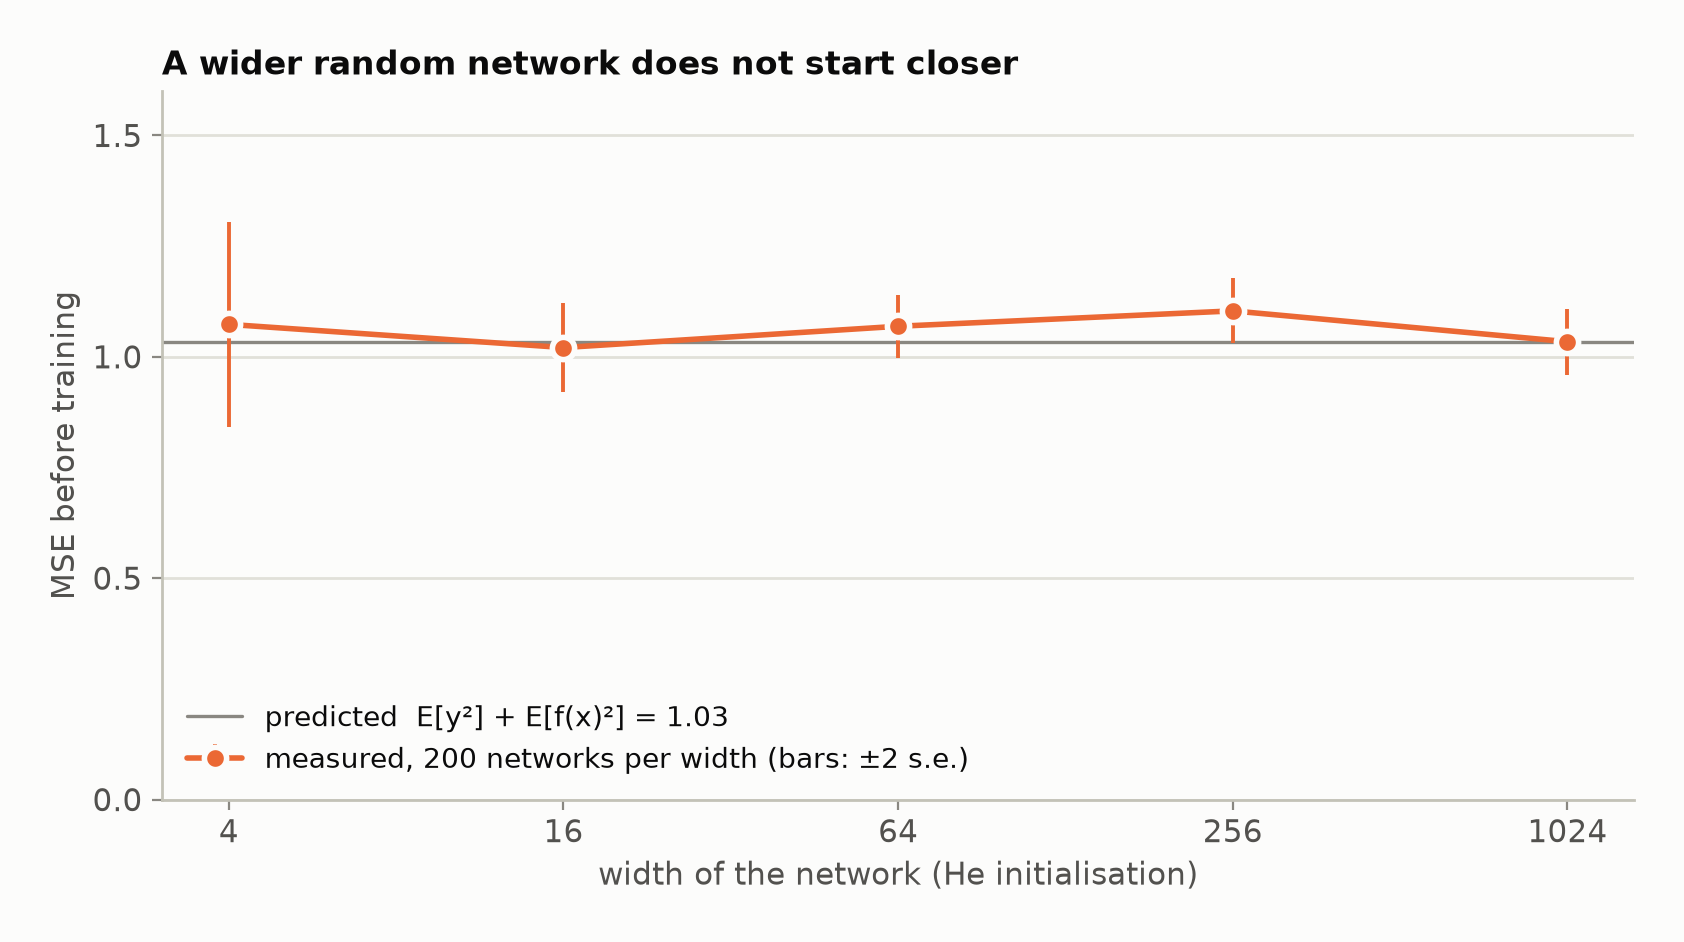
\includegraphics[width=0.74\linewidth]{../graphs/readme_initial_mse.png}
  \caption{Initial squared error of random ReLU networks under He
  initialisation (\cref{tab:mse}), with the prediction of \cref{cor:he}. Bars
  are $\pm2$ standard errors.}
  \label{fig:mse}
\end{figure}

\begin{table}[h]
  \caption{Random ReLU networks with a one-dimensional input: all sizes
  ($\pm$ one standard error over 300 networks; no training). Setup and caveats
  as in \cref{sec:nets}. Reference curves measured by the same code: the
  diagonal $y=x$ has length $2.83$ and distance $0.520$; a sine with one period
  across the box, $4.61$ and $0.351$; a sine with 16 periods, $64.07$ and
  $0.021$.}
  \label{tab:relu-full}
  \centering
  \begin{tabular}{rrrccc}
    \toprule
    width & hidden layers & parameters & arc length & turns & nearest-point \\
    \midrule
      2 & 2 &      12 & $3.446\pm0.040$ &  0.47 & $0.4808\pm0.0052$ \\
      4 & 2 &      32 & $3.571\pm0.037$ &  1.47 & $0.4540\pm0.0050$ \\
      8 & 2 &      96 & $3.512\pm0.034$ &  2.42 & $0.4398\pm0.0049$ \\
     16 & 2 &     320 & $3.604\pm0.035$ &  3.16 & $0.4231\pm0.0046$ \\
     32 & 2 &    1152 & $3.571\pm0.034$ &  4.39 & $0.4269\pm0.0046$ \\
     64 & 2 &    4352 & $3.559\pm0.035$ &  5.89 & $0.4269\pm0.0045$ \\
    128 & 2 &   16896 & $3.636\pm0.037$ &  8.18 & $0.4179\pm0.0046$ \\
    256 & 2 &   66560 & $3.577\pm0.036$ & 11.54 & $0.4286\pm0.0047$ \\
    512 & 2 &  264192 & $3.599\pm0.034$ & 15.11 & $0.4257\pm0.0046$ \\
    \midrule
     64 &  1 &    192 & $3.417\pm0.034$ &  3.05 & $0.4428\pm0.0047$ \\
     64 &  2 &   4352 & $3.613\pm0.037$ &  5.90 & $0.4256\pm0.0047$ \\
     64 &  3 &   8512 & $3.761\pm0.037$ &  8.39 & $0.4116\pm0.0048$ \\
     64 &  4 &  12672 & $3.900\pm0.039$ & 10.85 & $0.3938\pm0.0044$ \\
     64 &  6 &  20992 & $4.058\pm0.043$ & 15.67 & $0.3882\pm0.0044$ \\
     64 &  8 &  29312 & $4.368\pm0.049$ & 20.80 & $0.3643\pm0.0042$ \\
     64 & 12 &  45952 & $4.865\pm0.062$ & 28.88 & $0.3431\pm0.0040$ \\
     64 & 16 &  62592 & $5.100\pm0.075$ & 36.46 & $0.3433\pm0.0046$ \\
    \bottomrule
  \end{tabular}
\end{table}

\section{Lean names}
\label[appendix]{app:lean}

\begingroup\raggedright
The Lean project is in the folder \texttt{lean/} of the repository, built with
Lean 4.36.0-rc1 and the Mathlib commit recorded in
\texttt{lean/lake-manifest.json}. Each file is \texttt{lean/SquigglyLine/<name>.lean}.

\begin{itemize}\setlength{\itemsep}{1pt}
\item \cref{thm:sandwich}: \texttt{Sandwich}, \lean{nearestDist\_le\_verticalDist},
\lean{verticalDist\_le\_of\_lipschitz}.
\item \cref{thm:marginal} and \cref{cor:phase}: \texttt{Marginal},
\lean{expected\_residualLoss\_congr}; \texttt{RandomPhase},
\lean{marginal\_randomPhaseWave\_eq}; \texttt{Verdict},
\lean{not\_learningClaim\_sineWave}.
\item \cref{thm:tube}: \texttt{Coverage},
\lean{integral\_infDist\_eq\_integral\_uncovered}.
\item \cref{thm:cover}: \texttt{Oscillation},
\lean{nearestDist\_le\_of\_coversWithin},
\lean{verticalDist\_le\_of\_lipschitz\_of\_coversWithin},
\lean{expected\_nearestDist\_le}.
\item \cref{thm:sine}: \texttt{SineCloser},
\lean{sineWave\_nearestDist\_bounds},
\lean{tendsto\_expected\_nearestDist\_sineWave}; collected in
\texttt{SquigglyLineTheorem}, \lean{squiggly\_line\_theorem}.
\item \cref{prop:path,prop:more}: \texttt{LinearModel}, \lean{residual\_along},
\lean{exists\_within\_budget}, \lean{travel\_coprod\_le}.
\item \cref{thm:kernel}: \texttt{Kernel}, \lean{residual\_gradientStep},
\lean{travel\_eq\_norm\_of\_kernelInverse}, \lean{travel\_eq\_of\_kernel\_eq},
\lean{residual\_iterate\_gradientStep\_eq}.
\item \cref{cor:rate}: \texttt{ExchangeRate}, \lean{TightFeatures.travel\_eq};
\texttt{MarkovChains}, \lean{TightFeatures.residual\_iterate\_gradientStep},
\lean{TightFeatures.residual\_gradientStep\_inv}.
\item \cref{app:chains}: \texttt{NarrowChain}, \lean{narrowChain\_neverTurns};
\texttt{Depth}, \lean{iterate\_tent\_dyadic}; \texttt{Bridge},
\lean{sin\_sq\_iterate\_tent}; \texttt{Polarizer}, \lean{relu2\_nearest},
\lean{fan\_of\_le\_pi\_div\_two}, \lean{fan\_of\_pi\_div\_two\_le},
\lean{iterate\_fan}; \texttt{ThreePolarizers}, \lean{malus},
\lean{throughPlates\_light}, \lean{three\_polarizers},
\lean{quarter\_turn\_arrives}; \texttt{MarkovChains},
\lean{merged\_stays\_merged}, \lean{card\_image\_runLayers\_append\_le},
\lean{dead\_stays\_dead}.
\end{itemize}
\endgroup


\end{document}
